%%%%%%%%%%%%%%%%%%%%%%%%%%%%%%%%%%%%%%%%%%%%%%%%%%%%%%%%%%%%%%%%%%%%%%%%%%%%%%%%
%2345678901234567890123456789012345678901234567890123456789012345678901234567890
%        1         2         3         4         5         6         7         8

\documentclass[letterpaper, 10 pt, conference]{ieeeconf}  % Comment this line out if you need a4paper

%\documentclass[a4paper, 10pt, conference]{ieeeconf}      % Use this line for a4 paper

\IEEEoverridecommandlockouts                              % This command is only needed if 
                                                          % you want to use the \thanks command

\overrideIEEEmargins                                      % Needed to meet printer requirements.

%In case you encounter the following error:
%Error 1010 The PDF file may be corrupt (unable to open PDF file) OR
%Error 1000 An error occurred while parsing a contents stream. Unable to analyze the PDF file.
%This is a known problem with pdfLaTeX conversion filter. The file cannot be opened with acrobat reader
%Please use one of the alternatives below to circumvent this error by uncommenting one or the other
%\pdfobjcompresslevel=0
%\pdfminorversion=4

% See the \addtolength command later in the file to balance the column lengths
% on the last page of the document

\usepackage{cleveref}
\crefname{figure}{fig}{figs}
\usepackage{epsfig}
\usepackage{float}
\usepackage{threeparttable}
\usepackage{subfigure}

% The following packages can be found on http:\\www.ctan.org
%\usepackage{graphics} % for pdf, bitmapped graphics files
%\usepackage{epsfig} % for postscript graphics files
%\usepackage{mathptmx} % assumes new font selection scheme installed
%\usepackage{times} % assumes new font selection scheme installed
%\usepackage{amsmath} % assumes amsmath package installed
%\usepackage{amssymb}  % assumes amsmath package installed

\title{\LARGE \bf
Data-Efficient and Hardware  Decentralized Visual {SLAM}
}


\author{Jincheng Yu$^{1}$ and Feng Gao$^{1}$ % <-this % stops a space
% \thanks{*This work was not supported by any organization} % <-this % stops a space
\thanks{$^{1}$Electronic Engineering Department,
        Tsinghua University, Beijing, China
        {\tt\small yjc16@mails.tsinghua.edu.cn}}%
% \thanks{$^{2}$Bernard D. Researcheris with the Department of Electrical Engineering, Wright State University,
%         Dayton, OH 45435, USA
%         {\tt\small b.d.researcher@ieee.org}}%
}


\begin{document}

\maketitle
\thispagestyle{empty}
\pagestyle{empty}


%%%%%%%%%%%%%%%%%%%%%%%%%%%%%%%%%%%%%%%%%%%%%%%%%%%%%%%%%%%%%%%%%%%%%%%%%%%%%%%%
\begin{abstract}
Decentralized visual simultaneous localization and mapping (DSLAM) can share locations and environmental information between robots, which is an essential task for many multi-robot applications. For \textit{"robot"}, the Visual Odometry (VO) is a basic component to estimate the 6-DoF absolute pose, and for \textit{"multi"}, Decentralized Place Recognition (DPR) is a fundamental element to produce candidate place matches.
%Due to the advantages of Convolutional Neural Network(CNN) on image processing tasks, CNN-based VO and DPR have achieved significant improvements in performance., such as Depth-VO-Feat\cite{Zhan:2018e92} and NetVLAD\cite{Arandjelovic:2017997}. However, previous works concentrate on the accuracy of the CNNs, yet consider little about the deployment CNNs on the embedded system.
Although some CNN-based VO and DPR methods have made significant progress in performance compared to feature-based methods, such as Depth-VO-Feat \cite{Zhan:2018e92} and NetVLAD \cite{Arandjelovic:2017997}, they focus primarily  on the accuracy of CNNs, yet consider little about the deployment of CNNs on embedded systems.

Since the embedded system usually only supports fixed-point CNN, we propose a pose-sensitive fixed-point finetune method for the CNN-based monocular VO, and accelerate the per-frame VO from 230ms to 10ms with similar accuracy. In addition, empirical experiments show that the frequency of DPR has a large impact on the final result of DSLAM. So we propose a cross-component pipeline scheduling method to increase the computational speed of NetVLAD from once every 12 frames to once every 8 frames, and further improve the final accuracy of DSLAM.
% We find the tranditional average trajectory error (ATE) can not indicate the performance of trajectory merging in DSLAM, so we propose a new indicator called loop-closure recall (LCR) to evaluate the performance of trajectory merging.

% With the gradual improvement of the single-agent capabilities, it is possible to build up the multi-agent collaborative intelligence system.
% Distributed simultaneous localization and mapping (DSLAM) can share location and environmental information between robots and is the basis for many multi-agent applications.
% With the development of algorithms and computing platforms in recent years, convolutional neural network (CNN) has been widely used in SLAM systems, especially in visual-based SLAM systems.
% CNN can directly predict the pose with the absolute scale from two successive monocular frames, which can be easy to deploy on real robots and can make SLAM more robust in scenarios with pure rotations. Further, with CNN's versatility, it is easy to use the same network structure for many other tasks rather than depth or pose estimation, such as object detection and semantic segmentation.
% Finally, CNN's computational structure is uniform and can be individually optimized when resources are limited on embedded systems.

% In this work, we aim to build a fully CNN-based hardware-software co-design monocular DSLAM system. There are two keys components in DSLAM system: 1) Visual Odometry (VO) and 2) Place Recognition. We use fixed-point fine tune method to enhance the accuracy of CNN-based monocular VO and make it possible for acceleration on the Xilinx DPU accelerator. The same DPU also supports the place recognition component. We also propose a pipeline scheduling method to make full use of the DPU. To the best of our knowledge, this work is the first to implement all components of monocular DSLAM with CNN. We use the Xilinx ZU9 embedded MPSoC and the DPU IP core to validate the proposed DSLAM framework on the public dataset.
\end{abstract}

\section{Introduction}
\label{sec:introdutction}
In recent years, the capabilities of a single agent have been significantly improved. To further expand the capabilities of intelligent robots, using several robots can accelerate many tasks, such as localization, exploration, and mapping.
Decentralized visual simultaneous localization and
mapping (DSLAM) can share location and environmental information between robots and is the essential task for many multi-robot applications. \cite{Cieslewski:20187ee} concludes the basic procedure as \cref{fig:all}

\begin{figure}[h]  
    \centering  
    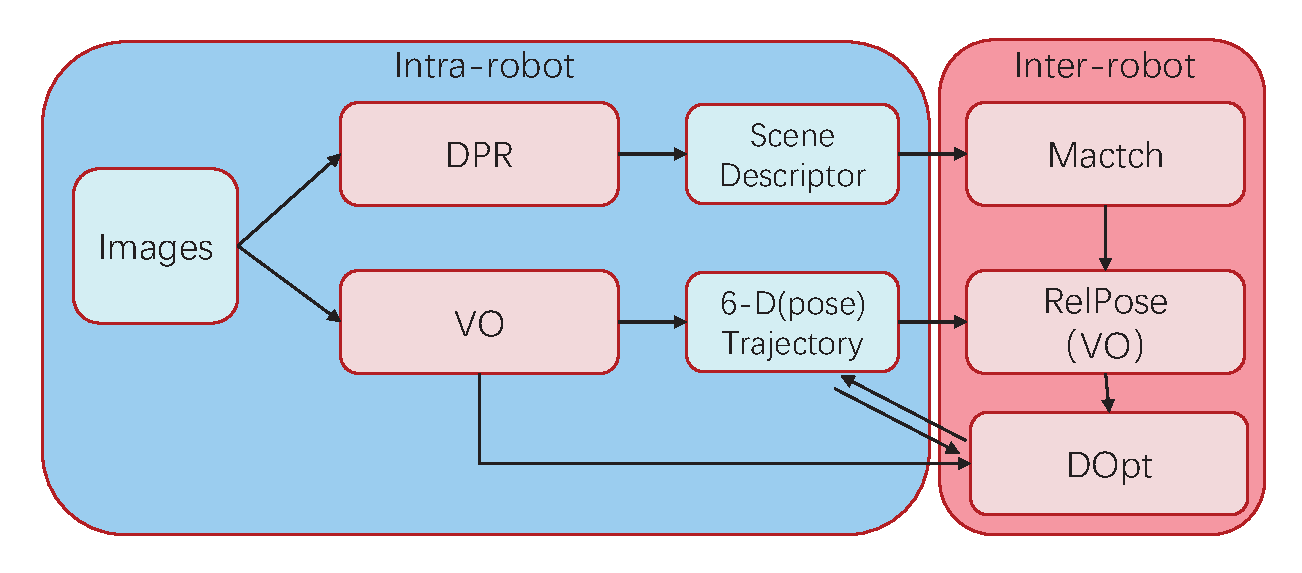
\includegraphics[width=0.75\linewidth]{fig/all.eps}
    \caption{DSLAM framework\cite{Cieslewski:20187ee}. \textbf{VO} is used to calculate the intra-robot 6-D absolute pose from the input frames. \textbf{DPR} produces a compact image representation that communicate among robots. \textbf{Match} stage finds out candidate inter-robot place recognition matches.  \textbf{RelPose} requires data from the matched robots and establishes relative poses between the robots trajectories. \textbf{DOpt} obtains the trajectories, intra-robot pose measurements from VO and inter-robot relative poses from RelPose, and updates the trajectories.}
    \label{fig:all}
\end{figure}

There are five components: DPR, VO, Match, RelPose and DOpt. DPR and VO are intra-robot operations, and require high computation resources on embedded system. Match, RelPose and DOpt are inter-robot operations, and consume most of the communication of DSLAM sytem. The RelPose components can and should depend the VO components since it can benefit from re-using the data and computation resources of VO.

The previous work \cite{Cieslewski:20187ee} uses ORB feature-point based method to estimate the trajectory from the sequence of the stereo camera, and use NetVLAD \cite{Arandjelovic:2017997} to do place recognition. These two algorithms both consume a large amount of computation and storage, and pose a great challenge to DSLAM on the embedded system. The DSLAM frame in \cite{Cieslewski:20187ee} is illustrated in \cref{fig:all_pre}.


\begin{figure*}[thb]
    \begin{minipage}[t]{0.5\linewidth}  
    \centering
    \subfigure[DSLAM in \cite{Cieslewski:20187ee}] {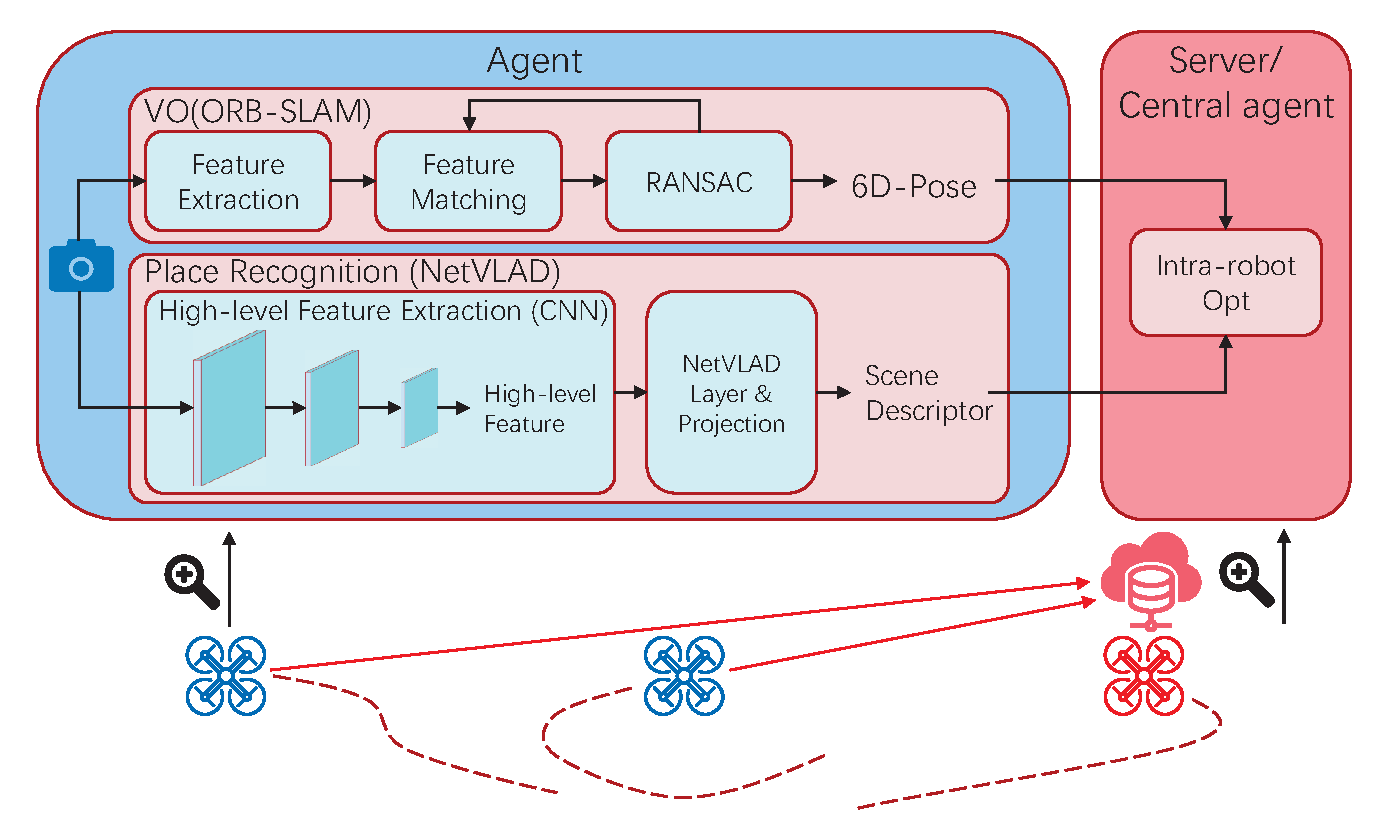
\includegraphics[width=0.8\textwidth]{fig/overview_pre.eps}\label{fig:all_pre}}
    \end{minipage}
    \begin{minipage}[t]{0.5\linewidth}  
    \centering  
    \subfigure[Our hardware-software co-design DSLAM.] {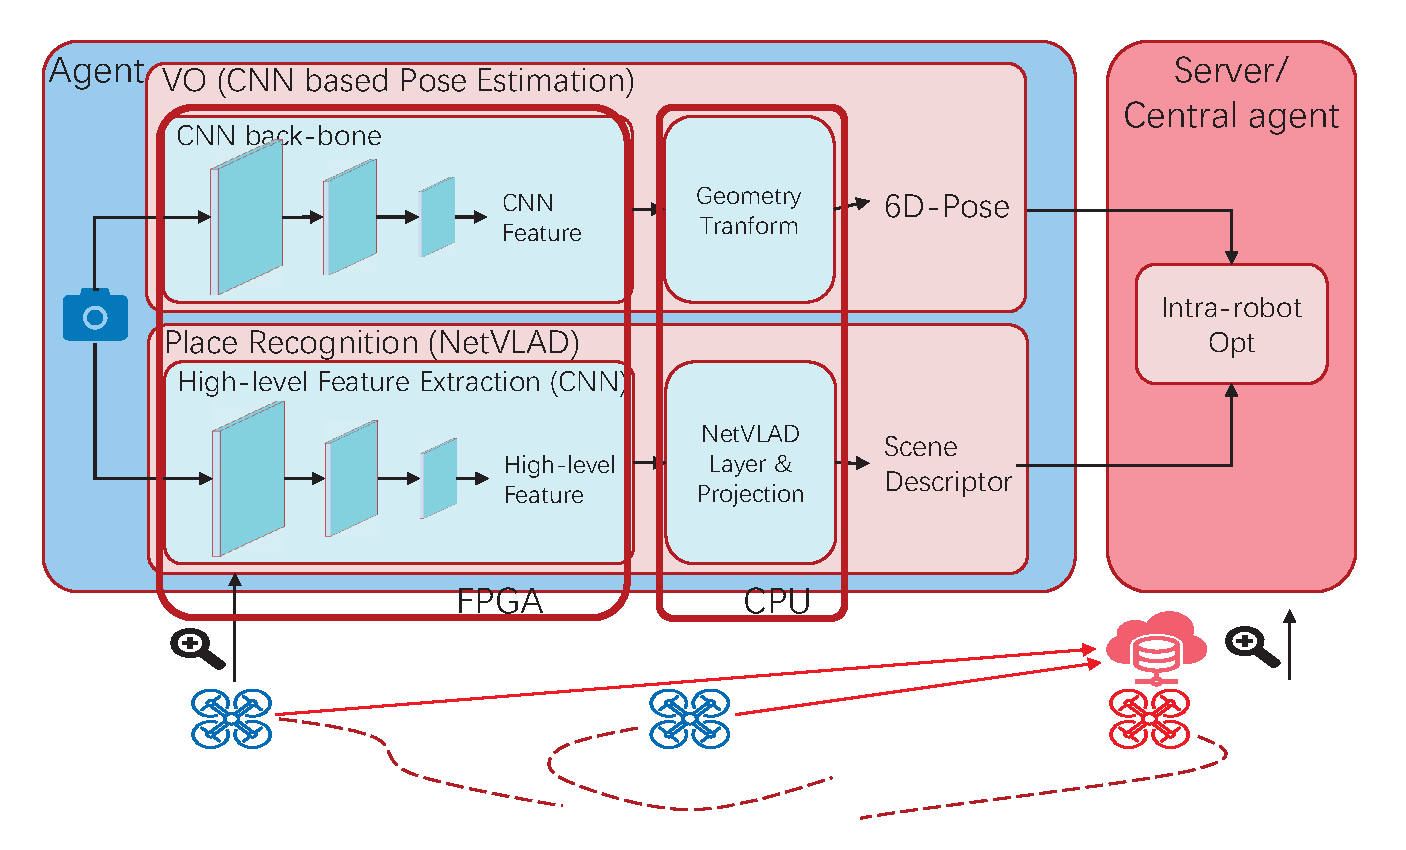
\includegraphics[width=0.8\linewidth]{fig/overview_us.eps}\label{fig:all_us}} 
    \end{minipage}
    \caption{???
    % Overview of the DSLAM in \cite{Cieslewski:20187ee} and our hardware-software co-design DSLAM. Each agent (blue drones) will send the result of 6-D pose estimation and scene descriptor to a server or a central agent (red server or drone in figure) to do inter-robot place recognition and optimization. We use CNN instead of feature points to do pose estimation so that we can use CNN accelerator to speed up the whole process.
    }
\label{fig:overview}
\end{figure*}

Monocular systems are much easier to deploy than binocular systems. The transitional monocular feature point based VO should use complex depth reconstruction methods to compute the absolute scale of the pose scale\cite{pizzoli2014remode}, leading to speed-down. With the development of CNN, we can reconstruct the depth and pose with the absolute scale from the monocular camera directly, making monocular VO more robust and efficient\cite{Zhan:2018e92}. ecent advances in deep learning and the availability of large labelled visual datasets have significantly improved the accuracy of place recognition, such as NetVLAD\cite{Arandjelovic:2017997}. However, previous works concentrate on the accuracy of the CNNs, yet consider little about the deployment CNNs on the embedded system.

Though DSLAM system can benefit from the development of CNN, the fully CNN-based DSLAM system faces some key issues: 1) The embedded system usually support fixed-point CNN. 2) The speed will decline in the embedded system when running several CNN models simultaneously, the speed-down of DPR will lead to the decline of the final DSLAM accuracy. Therefore, we build up a CNN-based monocular DSLAM system on embedded FPGA platform, with following contributions:

\begin{itemize}
\item To the best of our knowledge, this work is the first to implement all components of monocular DSLAM with CNN.
% We adopt Depth-VO-Feat \cite{Zhan:2018e92} in DSLAM system to estimate the pose from the input monocular camera. We use the same method of NetVLAD in  \cite{Cieslewski:20187ee} to do place recognition. 
We deploy the system on Xilinx Zynq MPSoC hardware platform with DPU \cite{Tech:2019360}, which is an embedded CNN accelerator. The proposed DSLAM framework is illustrated in \cref{fig:all_us}.
\item As the embedded system usually support fixed-point CNN, we propose a pose-sensitive fixed-point fine-tune method to make the feature extraction layers fixed-point and remain the pose prediction layers floating-point, reaching the same accuracy with the original floating-point VO network. We schedule the fixed-point layers on DPU and the floating-point layers on CPU, so that we can accelerate the VO to 10ms.
\item The frequency of the NetVLAD influences the final result of DSLAM. We propose a cross-components scheduling method to scheduling the computation flow across VO and DPR, and pipeline the computation across the PL and PS of MPSoC to make full use of the embedded platform. We calculate the NetVLAD every 4 input frames from every 6 frames, improving the final accuracy of DSLAM. 
We also propose a new indicator called loop-closure recall (LCR), which indicates the remaining rate of loop-closure after trajectory merging, to evaluate the performance of trajectory merging.
\end{itemize}

The output result of DSLAM with different NetVLAD frequency is illustrated in \cref{fig:dslamresult}. The tranditional average trajectory error (ATE) can not indicate the performance of trajectory merging in DSLAM. 

\begin{figure}[thb]
    \begin{minipage}[t]{0.475\linewidth}  
    \centering
    \subfigure[NetVLAD/8 frames. \protect\          ATE=0.9] {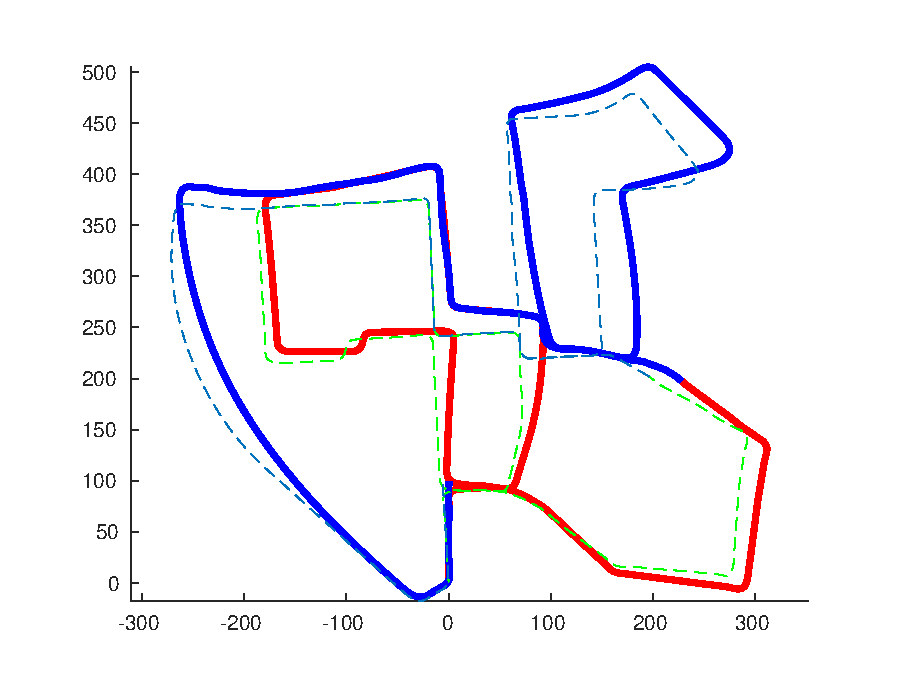
\includegraphics[width=1\linewidth]{fig/8netvlad.eps}\label{fig:8netvlad}}
    \end{minipage}
    \begin{minipage}[t]{0.475\linewidth}  
    \centering  
    \subfigure[NetVLAD/12 frames. \protect\ ATE=0.9] {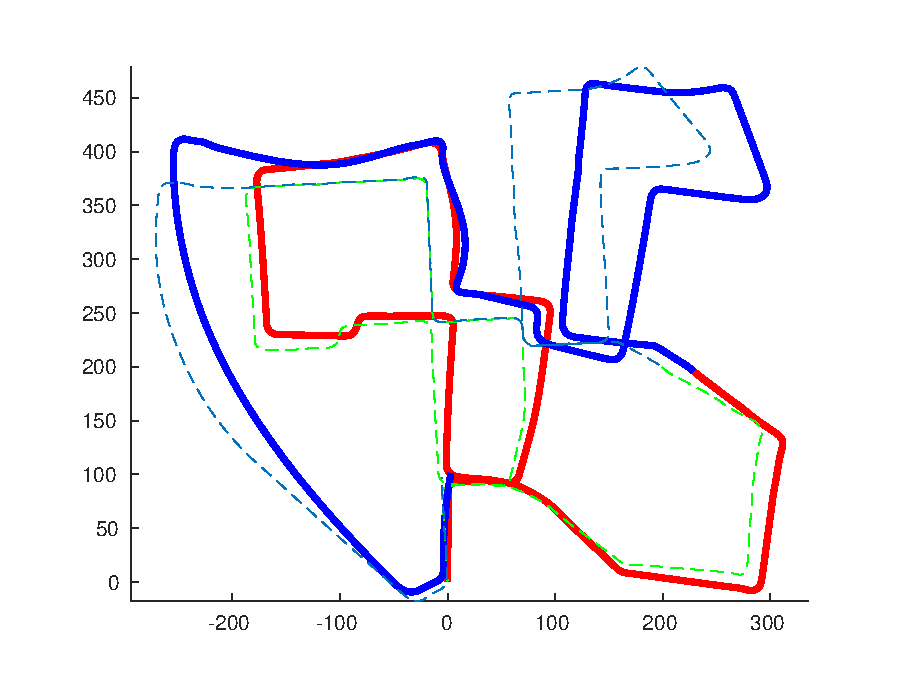
\includegraphics[width=1\linewidth]{fig/12netvlad.eps}\label{fig:12netvlad}} 
    \end{minipage}
    \caption{The result of DSLAM. \Cref{fig:8netvlad} do NetVLAD every 8 frames, and the frame con
    }
\label{fig:dslamresult}
\end{figure}



% The rest part of this article is orgnized as follows. \Cref{sec:background} will give the basic idea of CNN based methods and the hardware architecture of embedded platform, Xilinx Zynq MPSoC. \Cref{sec:hardsoft} will detail the implementation of our pose-sensitive fixed-point fine-tune method and the cross-components scheduling method. The experiment results will be given in \Cref{sec:experiment}. \Cref{sec:conclusion} will conclude this paper.

\section{Background}
\label{sec:background}
\subsection{CNN based methods in DSLAM}
As described before, there are two essential components on each agent: 1) Visual Odometry (VO) and 2) Place Recognition.

\subsubsection{Visual Odometry (VO)}

Visual odometry estimation is the task to infer ego-motion from a sequence of images and is an essential component in the SLAM system. Some feature-based SLAM systems have enjoyed great success, like ORB-SLAM\cite{DBLP:journals/trob/Mur-ArtalMT15} and ORB-SLAM2\cite{Mur-Artal:2017281}. Recently, several studies have shown that these feature-based SLAM systems require high computing resources. Fang et al.\cite{Fang2017FPGAbasedOF} shows that the feature extraction stage is the most computation-intensive, consuming over 50\% of the CPU resources.

As FPGA is one of the most promising platforms as the accelerator for VO, the SLAM system on FPGA has become a hot research topic. However, FPGA-accelerated feature extraction still consumes a lot of time and computing resources, which cannot be deployed simultaneously with an FPGA-accelerated neural network.

\subsubsection{Place Recognition}

The goal of place recognition is to calculate a given frame into a limited set of places. Each place can be encoded as a concise code which can be easy transferred with low communication cost. Traditional place recognition method usually translate the input frame as the aggregation of handcrafted feature point and local descriptors, like SIFT \cite{Lowe:2004e6e} or ORB \cite{Mur-Artal:2017281}, using vectorization techniques like bag-of-words (BoW) \cite{Galvez-Lopez:2012c94} or vector of locally aggregated descriptors(VLAD) \cite{Jegou:2010f45}.

Recent advances in the deep learning and the convolution neural network (CNN) enable powerful end-to-end mode for place recognition \cite{Noh:2017d0b, Arandjelovic:2017997}, and the NetVLAD method is one of the most accurate methods based on CNN. The NetVLAD algorithm based on VGG-16 model \cite{Simonyan:20143be} consumes more than $80G$ operations for a single $300 \times 300$ input image (each operation means addition or  multiplication). It is very challenging to deploy the NetVLAD on a traditional embedded hardware platform.

\subsection{Hardware architecture of Zync MPSoC}
The Xilinx Zync MPSoC is a chip with ARM cores and FPGA fabric. The system is illustrated in \cref{fig:plps}. The ARM cores with an embedded Linux operation system are called Processing System (PS). The FPGA fabric is called Programmable Logic (PL). The peripherals like camera and communication unit (WiFi or others) are accessible with PS. The high-bandwidth on-chip AXI interface is used to communicate between PS and PL. PS and PL can also share the DDR to transfer a large volume of data such as each frame of the camera.
Deephi CNN accelerator, which is called DPU \cite{Tech:2019360}, is one of the state-of-the-art accelerators and is famous for high energy efficiency on various CNN structure. We deploy the accelerator on the PL side of Zynq SoC with the help of DPU.

\begin{figure}[t]  
    \centering  
    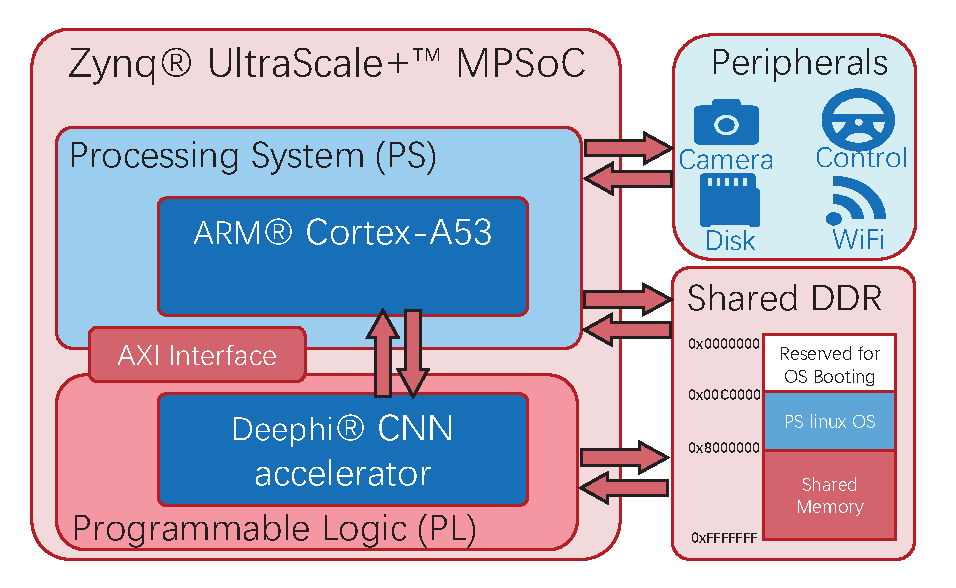
\includegraphics[width=0.95\linewidth]{fig/plps.eps}
    \caption{Hardware architecture of Zynq SoC}
    \label{fig:plps}
\end{figure}

Though FPGA can significantly improve the performance and energy efficiency of CNN inference, FPGA cannot efficiently calculate the floating-point number and requires fixed-point parameters and intermediate data in CNN.

\subsection{Motivation}
Though previous work \cite{Cieslewski:20187ee} proposes data-efficient DSLAM system, it is difficult to implement the two essential components, VO and place recognition simultaneously on a communication-limited and energy-constrained embedded hardware platform on a real robot. We propose this hardware-software co-design DSLAM system to use Xilinx Zynq MPSoC and Deephi DPU to execute these two components on the real system.



\section{Conclusion}
\label{sec:conclusion} 

We propose a hardware-software co-design DSLAM system with the help of Xilinx Zynq MPSoC and Deephi DPU. We optimize two essential components of DSLAM system,  1)Visual Odometry(VO) and 2) Place Recognition on the embedded system. From the aspect of calculation, the vectorization and projection operations on the PS side of Zynq MPSoC needed by NetVLAD is the bottleneck to do more frequent place recognition. From the aspect of communication, the data traffic for inter-robot relative pose estimation consumes the most communication resources. The accelerator for vectorization based on FPGA and more data-efficient inter-robot pose estimation method could be researched in future work.


\section*{Acknowledgment}
This work was supported by National Natural Science Foundation of China (Grant No.61874156)


\bibliographystyle{IEEEtran}
\bibliography{src/fpgaslam}

\end{document}
